
\section{Materiais Refratários Monolíticos}\label{mono}

Os materiais refratários são componentes fundamentais nas economias modernas
exercendo o papel de indústria habilitadora, no sentido em que possibilita a
execução de processos a elevadas solicitações térmicas, químicas e mecânicas em
um ambiente controlado e seguro. Ademais, o contexto sócio-ambiental do século
XXI exige a redução do desperdício de energia, especialmente em processos que
ocorrem a altas temperaturas, onde a perda de energia para o ambiente é
inerente.

Assim, a indústria de materiais refratários está diretamente ligada a setores
fundamentais como a de cimento e principalmente a siderúrgica, ambas estão
correlacionadas com o produto interno bruto (PIB) das nações
\cite{Ravazzolo2017, Bordigoni2016, Dobrota2013}, conforme demonstrado na Figura
\ref{fig:refractory_economy}.

\begin{figure}[!ht]
\centering
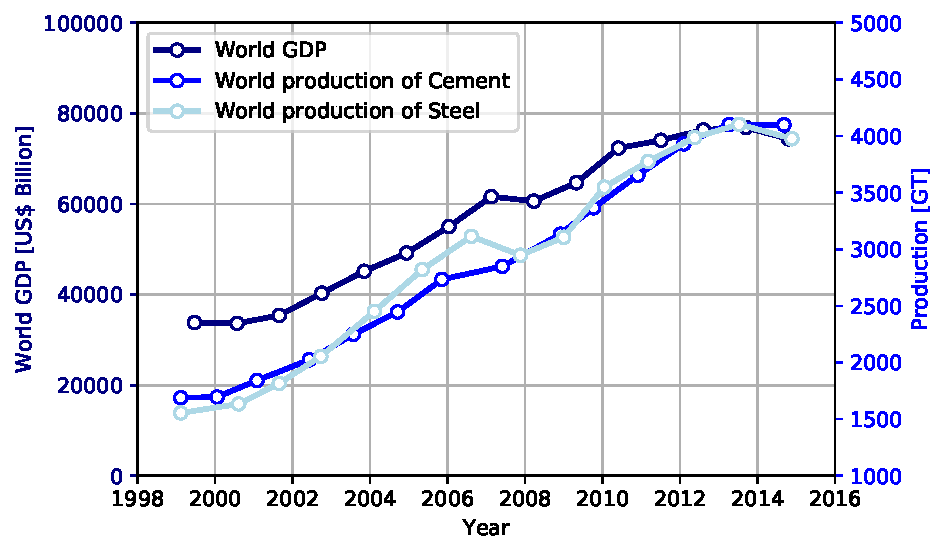
\includegraphics[width=\linewidth]{./figures/refractory_economy.pdf}
\caption{Evolução temporal do PIB mundial (azul escuro, eixo esquerdo), da
  produção mundial de Aço e Cimento (azul e azul claro, eixo direito) no período
  de 1999 a 2015. Adaptado de
  \cite{GlobalRef2017}. \label{fig:refractory_economy}}
\end{figure}

Com esse papel fundamental, os materiais refratários (que também são sujeitos a
processos em alta temperatura durante sua fabricação) também passam por uma
mudança de paradigma relativamente recente, isto é, ao invés do produtor
fornecer peças pré-formadas (refratários conformados), este passa a oferecer um
material conformável (monolítico), o que otimiza a logística - do ponto de vista
do produtor, evita e reduz estoques, reduz o custo energético e permite uma
maior customização do produto por parte do comprador. Dessa maneira, a seguir é
realizada uma breve revisão do conceito de materiais monolíticos, também
explorando seu processamento e finalmente as suas vantagens e desvantagens
características.

\subsection{Conceito}

A categoria de materiais monolíticos compreende materiais cuja etapa de
conformação não é realizada pelo produtor. Tal conceito ganhou força no contexto
do período entre guerras onde o foco era o ganho de produtividade
\cite{Schacht2004}. No geral cada uma de suas sub-classes se distinguem através
das diferentes metodologias de instalação, onde distintas propriedades reológicas
aliadas ao uso de ferramentas permitem a sua rápida conformação, diretamente no
equipamento a ser recoberto. A \autoref{tab:history} apresenta a evolução das
diferentes subclasses de materiais monolíticos.

\begin{table}[!h] 
\centering
\caption{Evolução do desenvolvimento de materiais refratários monolíticos, adaptado de \cite{Schacht2004}.}
\begin{tabular}{ccc}
\hline
Ano  & Desenvolvimento                                         & Tipo de instalação                    \\
\hline
\hline
1914 & Invenção da massas plásticas refratárias                & \textit{Ramming}     \\ \hline
1923 & Primeira patente de concreto refratário                 & \textit{Casting}     \\ \hline
1950 & Refratários projetáveis                                 & \textit{Dry Gunning} \\ \hline
1970 & Desenvolvimento de concretos defloculados               & Vibrado                               \\ \hline
1970 & Pré-fabricados                                          & Instalação Rápida                     \\ \hline
1980 & Refratários auto-escoantes                              & Auto-escoante                         \\ \hline
1990 & Refratários para  \textit{shotcreting} & \textit{Shotcreting} \\ \hline
\end{tabular}
\label{tab:history}
\end{table}

Os primeiros monolíticos desenvolvidos foram as massas plásticas, onde o uso de
um plastificante permite dar um formato bem definido a verde, que se mantém
coeso até sua queima. Em geral, os plastificantes utilizados são argilas
(especialmente as bentonitas sódicas - também conhecidas como bentonitas de
Wyoming) comuns no território americano \cite{bergaya2006general}, onde se deu
seu desenvolvimento \cite{Schacht2004}.
    
Em seguida, diversos desenvolvimentos em composições de concretos foram
alcançados permitindo as mais distintas formas de aplicação como \textit{Dry
  gunning}, vibração e \textit{Shotcreting}. Dentro da classe de materiais
monolíticos, os concretos foram uma das sub-classes que mais evoluíram
recentemente. Uma motivação para sua evolução é sua facilidade de aplicação que
aliada aos avanços em automatização gerou um interesse enorme em seu potencial,
além do seu alto desempenho \cite{Schacht2004}. Tal sub-classe compreende
materiais compostos, no geral, por agregados, uma matriz, ligantes, materiais
secundários e aditivos, o que torna o desenvolvimento de composições uma ciência
complexa e que também possibilita o ajuste de suas propriedades garantindo seu
uso nas mais distintas aplicações.
    
Os agregados formam o "esqueleto" do material e são as partículas de maior
tamanho (20 mm a 100 $\mu$m), sendo os componentes de maior
concentração dentro das formulações. A matriz é composta por materiais mais
finos (d < 100 $\mu$m) que objetivam maximizar o empacotamento da composição, enquanto o ligante
é o componente que confere a resistência mecânica. Os materiais secundários são,
geralmente,componentes mais baratos que também auxiliam na otimização do
empacotamento da composição, enquanto os aditivos são responsáveis a atribuir
características que possibilitem os mais diversos tipos de metodologia de
aplicação, como aceleradores e retardantes de pega, dispersantes e controladores
de pH.
    
A complexidade da formulação permite ajustes específicos que podem alterar as
propriedades finais do produto. Um exemplo é o uso de agregados leves e porosos
como uma maneira de redução da condutividade térmica, proporcionando um isolante
com alta resistência mecânica, ou ainda o uso de carbono como um material
secundário, que devido sua baixa molhabilidade por metais líquidos aumenta a
resistência a corrosão do produto \cite{Schacht2004}.
    
Outro fator importante da formulação, e que recentemente passou a definir
inclusive quais as quantias de cada fração granulométrica, é o seu grau de
empacotamento. Como a resistência aos ambientes altamente reativos é um
requisito fundamental dos materiais refratários, a redução da porosidade foi uma
das grandes motivações que levaram a consideração de teorias de empacotamento
para o ajuste da formulação uma vez que a porosidade aberta aumenta a área
superficial do material em contato com o ambiente agressivo. Dentre as
principais, listam-se a teoria de empacotamento de Alfred e o modelo de
Andreasen \cite{Ortega1997}.
    
Tais avanços permitiram o desenvolvimento de materiais com resistência mecânica
otimizada. Entretanto, um dos grandes contrapontos à maximização do
empacotamento se dá na etapa de secagem do material. Especialmente em concretos
com ligações hidráulicas (como sistemas com cimento de aluminato de cálcio,
CAC), reações de desidratação passam a ocorrer na faixa de 210$^\circ$C à
370$^\circ$C, o que pode gerar vapores aprisionados na estrutura pouco
permeável das composições de empacotamento otimizado, sendo possível que os
níveis de pressão alcançados nessas regiões sejam maiores que a resistência
mecânica do material levando ao trincamento, lascamento, que reduzem a vida útil
do revestimento, e até mesmo explosões, que podem comprometer a integridade de
todo o equipamento. Assim, a próxima seção traz as principais estratégias
adotadas pelas indústrias nos esforços de otimização da secagem e como a
simulação computacional poderia complementar tais estratégias.
 

%%% Local Variables:
%%% mode: latex
%%% TeX-master: "TCC-Secagem"
%%% End:
